To be able to model the prepayment risk for the lender, the behavior of 
the borrower will be modelled based on given data. In this report
the open source data provided by FreddieMac will be used (\cite{FredieMac}). This data set contains mortgage information of the bank FreddieMac over the time
interval start 2013 until september 2020. In general the data set is anonymized.
This will mean that there will be no personal information within the data set.
However, data that cannot be referred to the specific persons in the data set
will be included.
\\\\
As the data contains the information of the clients of the FreddieMac bank, in 
the report, the borrower will be referred as clients. In general the report will 
address all the data provided by FreddieMac as 'the data set'. Moreover, the 
data set can be distinguished into two categories. First of all there is data 
with respect to the moment the mortgage is closed. This data is not time 
dependent and will be referred to as the originate data. On the other hand 
there is the data that corresponds to the monthly developments of the 
mortgages. This part of the data set will be referred to as the monthly 
data.
\\\\
To extract meaningfully information from the data set, the report addresses 
the data analysis in several steps. First the report will go in some 
further depth on what is in the data set. After this, the report will 
continue with some elaboration about the way the data will be cleaned. 
From the cleaned data, the prepayment categories can be derived. Using the 
found prepayment categories, the risk drivers for the prepayment risk 
will be distinguished both on the originate data as on the monthly data.  

\subsection{Data description}
    The data collected by FreddieMac consist of different files. 
    For each year, there is a given originate data file and a monthly 
    data file. FreddieMac continuously 
    updates and corrects the files to keep them up to date. 
    In this report, not the total data set of the FreddieMac open source 
    set is used. 
    A sample of the data over the years (february) 2013 until (september) 2020 
    is used. For each year the sample contains approximately 50000 loans.
    Only the year 2020 does not contain that many loans, as this data is 
    not from a full year.
    The originate data consists of 31 characteristics of a loan:
    \begin{itemize}
        \item credit score (which will be referred as "FICO"), 
        \item first payment date, 
        \item first time home buyer flag, 
        \item maturity date, 
        \item Metropolitan statistical area (which will be referred as "MSA"), 
        \item mortgage insurance percentage,
        \item  number of units, 
        \item occupancy status, 
        \item original combined loan-to-value (which will be referred as "CLTV"), 
        \item original debt-to-income rate (which will be referred as "DTI"), 
        \item original UPB, 
        \item original loan-to-value (which will be referred as "LTV"), 
        \item original interest rate, 
        \item channel, prepayment penalty mortgage flag 
        (which will be referred as "PPM"), 
        \item amortization type, property state, 
        \item property type, postal code, 
        \item loan sequence number, 
        \item loan purpose, 
        \item original loan term, 
        \item number of loanees, 
        \item seller name, servicer name, 
        \item super conforming flag, 
        \item pre-HARP loan sequence number, 
        \item program indicator HARP indicator, 
        \item property valuation method,
        \item interest only indicator.
    \end{itemize} 
    For a much more detailed explanation of all those characteristics 
    the reader can be referred to the User Guide provided by FreddieMac (\cite{FredieMac}). 
    % 
    % We need some reference here. 
    % 
    \\\\
    Additional to the originate data file, the monthly performances
    are also combined in a file per year. This "monthly performances file" 
    consist of the monthly development of the mortgages.  
    This data is therefore dependent on time and thus yields the monthly 
    information about the development of the loan. 
    The data of every loan is monthly determined from the first payment 
    date until september 2020. If the mortgage is fully repaid due to 
    full prepayment at some date or the maturity date is reached, 
    there will not be any more data of that loan available after this date.  
    The monthly performance file consist of 30 characteristics: 
    \begin{itemize}
        \item Loan sequence number,
        \item monthly reporting period, 
        \item current actual UPB, 
        \item current loan 
        \item delinquency status, 
        \item loan age, 
        \item remaining months to legal maturity, 
        \item repurchase flag, 
        \item modification flag, 
        \item zero balance code, zero 
        \item balance effective date, 
        \item current interest rate, 
        \item current deferred 
        \item UPB, 
        \item due date of last pain instalment (which will be referred as "DDLPI"), 
        \item MI recoveries, 
        \item net sale  proceeds, 
        \item non MI recoveries, 
        \item expenses, 
        \item legal costs, 
        \item maintenance and preservation costs, 
        \item taxes and insurance, 
        \item miscellaneous expenses, 
        \item actual loss calculation, 
        \item modification cost, 
        \item step modification flag,
        \item deferred payment plan,
        \item estimated loan to value (which will be referred as "ELTV"), 
        \item zero balance removal UPB, 
        \item delinquent accrued interest, 
        \item delinquency due to disaster, 
        \item loanee assistance status code
    \end{itemize}
    Also here, For a much more detailed explanation of all those characteristics,
    the reader can be referred to the User Guide provided by FreddieMac.
    \\\\        
    Not all these characteristics are that relevant to predict a prepayment of the 
    client in the future and some can therefore be removed from the data. 
    Details on which characteristics will be removed and the corresponding 
    reason for removing these characteristics will be given in the next subsection.

\subsection{Data cleaning}
    As the data set contains much information about all kinds of mortgages 
    and clients, not all characteristics and specific mortgages will be 
    useful for predicting the prepayments. For example, missing data and 
    mortgages from which the outstanding debt is set to zero based on some 
    administrational reason are not useful for predicting the prepayment 
    probabilities. Hence this data will be removed from the data set. The 
    process of removing not useful data will be referred as "data cleaning". 
    \\\\  
    At first, all columns with no values at all can be removed. 
    The characteristics for which no data is provided in the data are: 
    \begin{itemize}
        \item pre-HARP
    	\item Harp indicator
    	\item Interest only indicator
        \item mi recoveries
        \item net sale proceeds
        \item non mi recoveries
        \item expenses
        \item legal costs
        \item maint pres costs
        \item taxes ins costs
        \item misc costs
        \item actual loss
        \item deliquent accrued interest
    \end{itemize}
    Besides the specific characteristics which do not have useful data 
    to work with, also the mortgages from which not all data is provided
    (or is reliable) will be removed. 
    Mortgages that meet the following conditions, are removed. 
    % fico == 9999
    % Original Combined Loan-To-Value == 999
    % Original Debt-To-Income Ratio == 999
    % Original Loan-To-Value == 999
    % Product type == _
    % Prepayment penalty == ""
    % Zero balance code > 1
    \begin{itemize}
        \item The FICO is not known.
        \item The CLTV is not known.
        \item The debt to income ratio is not known, 
        \item The original loan to value is not known, 
        \item The product type is not known, 
        \item The prepayment penalty is not known, 
        \item The zero balance code is greater than one (this 
        includes all loans that were administrational set to zero, 
        when no prepayment occurred).  
    \end{itemize}
    As there is only interest for 
    prepayment or matured mortgages, the data is filtered on the 
    zero-balance code. The zero-balance code is a code implying what 
    happened to the mortgage. A total of 373602 loans fitted to 
    predict prepayments is obtained, see Table 
    \ref{model_cleaned data_table} for the distribution over the 
    years. 
    \begin{table}[H]
        \centering
        \begin{tabular}{c|c}
            Year & Number of loans \\\hline
            2013 & 49835 \\
            2014 & 49821 \\
            2015 & 49871 \\
            2016 & 49878 \\
            2017 & 49836 \\
            2018 & 49841 \\
            2019 & 49698 \\
            2020 & 24822 \\\hline
            Total & 373602 
		\end{tabular}
		\caption{
            Number of loans for years 2013-2020 after 
            cleaning the data. As the there is only 
            data available for 2020 until september, 
            the total amount of loans is a bit lower for 
            2020. 
            }
		\label{model_cleaned data_table}
    \end{table}
    
\subsection{Prepayment derivation}
    The prepayment is defined as repaying the more of the outstanding debt 
    than was scheduled in the agreement. 
    Hence, first the payment schedule has to be derived. 
    
    \subsubsection{Obtain monthly payments in annuity mortgage}
        Let $t_0$ be the moment at which the mortgage is closed.
        Set $t_1$ equal to the first moment the client will repay a 
        part of the outstanding debt. 
        Let $t_n$ be the moment that the client will repay the last 
        part of the outstanding debt. This moment can be derived 
        from the first payment date and the loan term.
        As a consequence, there will be $n$ payments. 
        The payment schedule is given by payments:
        \begin{equation}
            B_{t_0}, \ldots, B_{t_n}
        \end{equation}
        over the moments $t_0, \ldots, t_n$. 
        An annuity mortgage is characterize by its equal payments.
        Hence the payments have the relation $B \equiv B_{t_j}$ for 
        $j \in \{0, 1, \ldots, n\}$. 
        Note that at $t_0$ there is no payments (as the mortgage is granted).
        Let us denote the interest at time $t$ as $r_t$ for some time 
        $t$. 
        Since fixed mortgages are considered, the relation $r \equiv r_t$ 
        holds for the interest rates. 
        Assume a risk neutral market. 
        When the loan is priced in the risk 
        neutral market, the present value of the outstanding debt, should be 
        equal to the loan at time $t_0$. Hence the relation,
        \begin{equation}
            L = B (1 + r)^{-t_1} + \ldots B (1 + r)^{-t_n}
        \end{equation}
        where $L$ is the granted loan, should hold. 
        Using the geometric series, the value of each payment 
        $B$ can be determined: 
        \begin{equation}
            B\left[
                \displaystyle\sum_{j=1}^{n} \left(
                    (1 + r)^{-1}
                    \right)^{t_j}  
            \right] = 
            B\left[
                \displaystyle\sum_{j=0}^{n} \left(
                    (1 + r)^{-1}
                    \right)^{t_j} - 1  
            \right] = 
            B \left[
                \dfrac{
                    1 - \left(
                        \dfrac{1}{1 + r}
                    \right)^{n+1}
                    }
                    {
                        1 - \dfrac{1}{(1 + r)}
                    } - 1
            \right].
        \end{equation}
        From this the monthly payments $B$ can be determined: 
        \begin{equation}
            B = \dfrac{L}{
                    \left[
                        \dfrac{
                            1 - \left(
                                \dfrac{1}{1 + r}
                            \right)^{n+1}
                            }
                            {
                                1 - \dfrac{1}{(1 + r)}
                            } - 1
                    \right]        
                }
        \end{equation}
        The term 
        \begin{equation}
            \dfrac{
                1 - \left(
                    \dfrac{1}{1 + r}
                \right)^{n+1}
                }
                {
                    1 - \dfrac{1}{(1 + r)}
                } - 1
        \end{equation}
        will be called the monthly factor. 
        Note that the interest rate given is a yearly based interest rate. 
        The corresponding monthly rate can be calculated by: 
        \begin{equation}
            (1 + r)^{\frac{1}{12}}.
        \end{equation} 

        The outstanding debt $U_{t_j}$ at time $t_j$ is now given by,
        \begin{equation}
            U_{t_j} = B \left(
                (1+r)^1 + (1 + r)^2 + \ldots + (1 + r)^{t_n - t_j}
                \right)
        \end{equation}
        where $t_n$ is the last payment date. This yields a payment of the 
        UPB at time $t_j$ of
        \begin{equation}\label{upb_part}
            U_{t_{j-1}} - U_{t_{j}} = 
            B (1 + r)^{t_n - t_j + 1}  
        \end{equation}
        Using the payment schedule and the corresponding derivation of 
        the repaid non-interest rate bearing part, the prepayments 
        can be classified in the data. 
 
    \subsubsection{Prepayment in the data}
        Using the monthly data, the loan term and the original UPB, 
        the payment schedule can be derived on a monthly basis. 
        Using the scheduled payments and expression \eqref{upb_part}, 
        the scheduled repayments of the UPB can be derived and 
        computed on a monthly basis.
        Denote the scheduled repaid UPB part at time $t_j$ as 
        $\hat{P}_{t_j}$ and denote the actual repaid UPB part 
        as $P_{t_j}$. Set a threshold percentage $\alpha$ 
        to deal with some minor variations in $P_{t_j}$.
        Now define the following mapping: 
        \begin{equation}
            \ppmFlagA = \left\{
                \begin{array}{l l l l l }
                    1 & \text{if} &
                    P_{t_j} > (1 + \alpha) \hat{P}_{t_j} \\ 
                    0 & \text{else}
                \end{array}
            \right.
        \end{equation}
        Using this mapping, a flag for the prepayments can 
        be set. Then, if the full outstanding debt is paid
        and $\ppmFlagA = 1$, then there is a full prepayment. 
        Otherwise, if $\ppmFlagA = 1$ and the current 
        UPB is greater than zero, it will be addressed as a 
        partial prepayment. If $\ppmFlagA = 0$ then 
        there is no prepayment. It is known that for the 
        first 6 months the payment data is not reliable. 
        Hence, $\ppmFlagA$ is adjusted for this. Only 
        $P_{t_j}$ with $t_j > 6$ are included in the 
        categorization of the prepayments. 
        In the data, there is also an adjustment for delinquent 
        clients, which have a default before $t_j$. 
        Denote the delinquency status $d_{t_j}$ as
        \begin{equation}
            d_{t_j} = \left\{
                \begin{array}{l l l l l}
                    1 & \text{if} & \text{there is a default at } t_j \\
                    0 & \text{else}
                \end{array}
            \right.
        \end{equation}
        Denote the cumulative delinquency status at $t_j$ as:
        \begin{equation}
            D_{t_j} = \displaystyle\sum_{k=1}^{j} d_{t_k}.
        \end{equation}
        Hence, if 
        there is a default before time $t_j$ the adjusted 
        $\ppmFlag$ is obtained as: 
        \begin{equation}
            \ppmFlag = \left\{
                \begin{array}{l l r l l }
                    1 & \text{if} & D_{t_j} > 0 & \text{and} &
                    P_{t_j} > 2(1 + \alpha) \hat{P}_{t_j} \\ 
                    1 & \text{if} & 
                    P_{t_j} > 2(1 + \alpha) \hat{P}_{t_j} \\ 
                    0 & \text{else}
                \end{array}
            \right.
        \end{equation}
        Using the $\ppmFlag$ and the amount of the outstanding
        the prepayments can now be classified.  
        In Table 
        \ref{model_classficationprepayment_table}, the number of 
        loans with prepayments are given. 
        From this table it can be seen that 
        loans consisting of no prepayments or full prepayments 
        are appearing most in the sample data.
        \begin{table}[H]
        \centering
            \begin{tabular}{c|c|c|c|c}
                & \multicolumn{4}{c}{Number of loans} \\
                Year&No Prepayment&Partial Prepayment&Full Prepayment &Both Partial \& Full prepayment  \\\hline
                2013 & 20783 & 4159 & 22136 & 2757\\
                2014 & 17909 & 3082 & 26537 & 2293\\
                2015 & 24027 & 3365 & 20811 & 1668 \\
                2016 & 28984 & 3137 & 16603 & 1154 \\
                2017 & 29460 & 2479 & 16959 & 938 \\
                2018 & 27368 & 1764 & 19901 & 808 \\
                2019 & 37041 & 1049 & 11426 & 182 \\
                2020 & 24160 & 39 & 623 & 0 \\\hline
                Total & 209732 & 19074 & 134996 & 9800
		    \end{tabular}
		    \caption{Classification of loans for years 2013-2020 with 
            threshold percentage of $\alpha = 0.1$. 
            The last column corresponds with the amount of 
            clients that do both at least one partial prepayment and a 
            full prepayment.}
		    \label{model_classficationprepayment_table}
        \end{table}
        Furthermore, it is noted that there are relative few 
        prepayments. For example in the year 2013, the percentage 
        of prepayments with respect to all considered loans in that year
        is approximately
        \begin{equation}
            \dfrac{
                22136  
            }{
                49835
            } \approx 0.44,
        \end{equation}
        which is almost 44 percent. From this it can be suggested that 
        prepaying is not a rare event. As this is a sample of a greater 
        data set provided by FreddieMac, this result should be compared 
        with the greater data set. Within this report, it is assumed that
        the sample is representative for the whole data set.  
        \\\\ 
        From the previous table, it can also be seen that the number of 
        prepayments (partial and full) decrease over time. This 
        phenomena is due to the time dependence of the prepayment 
        incentive of the client. As both the client's and the macro 
        economic circumstances change over time, the incentive for 
        the client to prepay will  be time dependent. Hence it is 
        expected that there are fewer prepayments at a time step $t_j$ 
        close to $t_0$ and the number of prepayments increase over 
        time. The number of prepayments is a cumulative count, and hence 
        will only increase. As a consequence, portfolios containing 
        mortgages that were closed earlier in time (for example 2013)
        will contain more prepayments than portfolios containing more 
        recent mortgages (for instance 2019). This time dependence is 
        also a phenomena that should be addressed in the modelling.
        For this reason, it is assumed that for a total portfolio 
        the number of prepayments over a specific time interval is 
        equal upon an random error with expected value zero.
        
        %
        % Some picture here
        % \textcolor{red}{Picture over the years!}
        %

\subsection{Importances of the data}
    Before addressing the possible drivers of the prepayment risk, 
    first a note is placed with the available data.  
    As the data set is anonymized, some characteristics of the loans and 
    clients are made general and hence could be more difficult to work with. 
    Some drivers for the risk of prepayment could be 
    for instance the age and the income of a certain client. 
    Someone with a 
    higher income is more likely to prepay, similarly, someone older is 
    more likely to have some extra money and therefore has a higher 
    probability to prepay. 
    However, these sort characteristics are not directly available in the 
    data.
    For instance,
    income is used to calculate several measures which are included in the
    data, but not given specifically. 
    Moreover, age is never mentioned in the data although it 
    may be useful for predicting prepayments or simulating other 
    characteristics over time.  
    \\\\
    In the remainder of this section, the possible risk drivers 
    for the prepayment risk will be discussed. Among these drivers, 
    there are drivers that were derived from the personal information
    of the client (e.g. the LTV) and some macro economic drivers. 
    Only a small selection of characteristics is discussed, other 
    characteristics behave similar in cases of no prepayment and 
    prepayment. 
    A more general approach of variable selection will  be discussed 
    in Section \ref{section_model}, where the LASSO approach will
    be discussed. 
    
    \subsubsection{Original unpaid principal balance}
        An important characteristic of a loan is the UPB.
        The UPB considers the non-interest bearing part of the 
        outstanding debt.  
        This characteristic 
        is used to calculate both LTV and CLTV. From the 
        observations of CLTV and LTV it is expected that a loan 
        with high UPB with small purchase price is more likely 
        to be prepaid. This will be discussed in the next section. 
        On the other hand, a low UPB is also likely to be 
        prepaid as the money required to make a prepayment is 
        less in comparison to a high UPB. To see if this is in 
        accordance with the data a boxplot consisting all 
        sorts of prepayments is formed. This boxplot contains 
        data of all the years.  In Figure 
        \ref{model_boxplot_UPB} one sees the UPB corresponding 
        to partial prepayments to be smaller than the UPB of no 
        prepayments. Which is in accordance with our last remark 
        about the behavior of the UPB. On the other hand, the 
        UPB corresponding to full prepayments turns out to be 
        higher than the UPB of no prepayments. This is also 
        observed in the behavior of LTV and CLTV (see 
        for example Section \ref{orig_ltv}). 
        \begin{figure}[H]
            \centering
            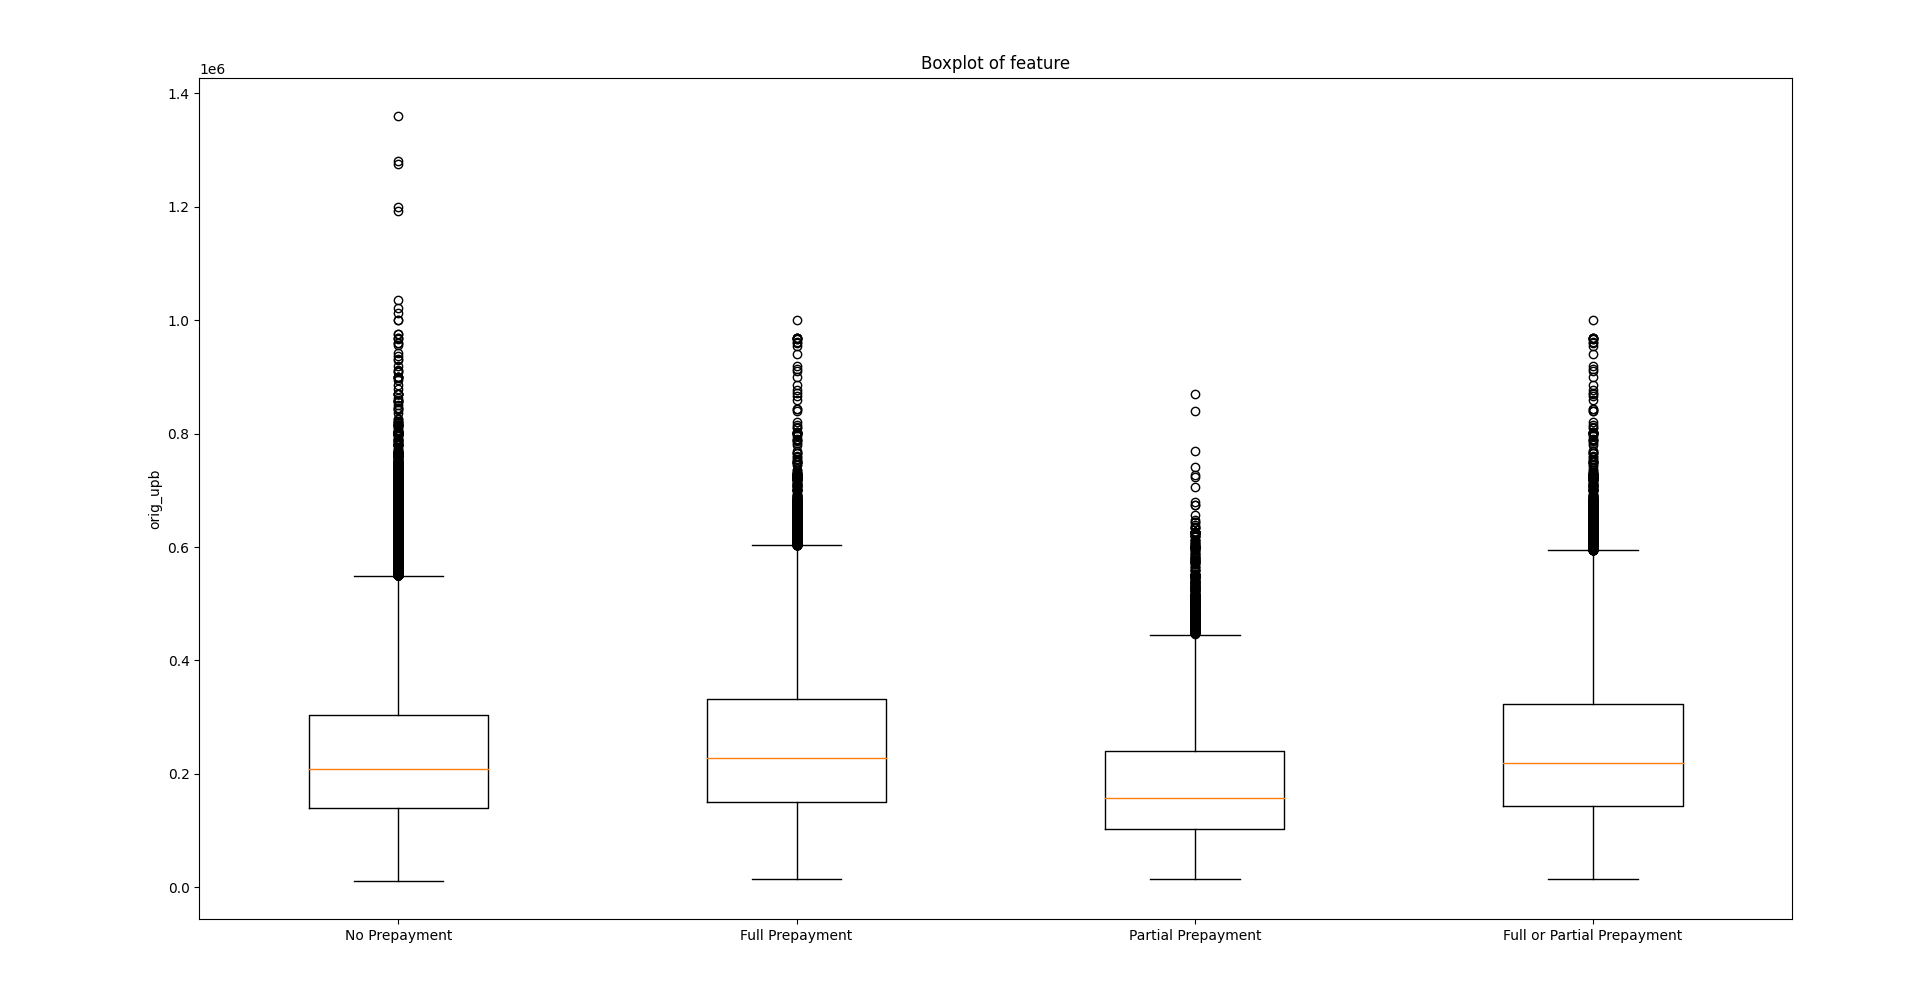
\includegraphics[width=\linewidth]{Figures/Boxplot_of_upb_[2013, 2014, 2015, 2016, 2017, 2018, 2019, 2020]_.png}
            \caption{
                Boxplot of UPB for sample data. From left to right: 
                No prepayment, Full prepayment, Partial prepayment 
                and Full or Partial prepayment.
                }
            \label{model_boxplot_UPB}
        \end{figure}
        \noindent
        A two sample Kolmogorov Smirnov test (KS-test) is used to
        determine wheter prepayment data is drawn from the same
        distribution. The null hypothesis states that two samples are drawn from the same continuous distribution. A small $p$-value rejects the null hypothesis, while a large $p$-value does not reject the null hypothesis. The two sample KS-test makes use of a two sided alternative hypothesis. 
        
        In Table \ref{model_Pvals_of_UPB}, all $p$-values are zero and hence 
        the two samples are considered from different from different 
        distributions concerning the UPB. One have to note that in case of much data points 
        the null hypothesis is more often rejected then for less data points. 
        Hence too much data could also explain these $p$-values. 
        \begin{table}[H]
        \centering
            \begin{tabular}{lcl|c|c}
                \multicolumn{3}{c|}{Prepayment type} 
                & P-values& KS-statistic \\\hline
                No Prepayment & \& & Full Prepayment & 0 & 0.068385\\
                No Prepayment & \& & Partial Prepayment & 0 & 0.182088\\
                No Prepayment & \& & Full or Partial Prepayment & 0 & 0.043719 \\
                Full Prepayment & \& & Partial Prepayment & 0 & 0.238933
		    \end{tabular}
            \caption{
                $p$-values of UPB (in which if both partial and full 
                prepayments happen, it is denoted as full prepayment).
                }
	        \label{model_Pvals_of_UPB}
        \end{table}
        For all years separately, similar results are obtained.
        It therefore suffices to just look at one year.  
        By isolation the data of year 2013, Figure 
        \ref{model_UPB_against_prepayment} is obtained. Here a smaller 
        UPB results in more prepayments. Hence, UPB is an 
        important characteristic to predict prepayments. 
        \begin{figure}[H]
            \centering
            \begin{subfigure}{0.45\textwidth}
                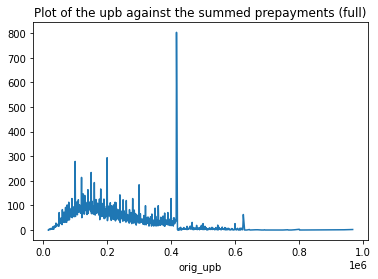
\includegraphics[width=\linewidth]{Figures/UPB againts Full prepayments.png}
                \caption{
                    UPB against Full prepayments.
                    }
                \label{model_UPB_against_full_prepayment}
            \end{subfigure}
            \begin{subfigure}{0.45\textwidth}
                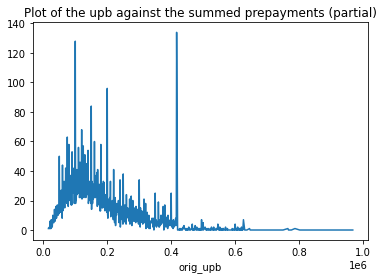
\includegraphics[width=\linewidth]{Figures/UPB againts Partial prepayments.png}
                \caption{
                    UPB against Partial prepayments.
                    }
                \label{model_UPB_against_partial_prepayment}
            \end{subfigure}
            \caption{
                UPB against magnitude of prepayments.
                }
            \label{model_UPB_against_prepayment}
        \end{figure}


    \subsubsection{Original loan-to-value}\label{orig_ltv}
        Some characteristics of a loan are based on the same information
        and will therefore by likely to be dependent. 
        For example, both LTV and CLTV 
        are both calculated using the original loan amount
        (which refers to the outstanding debt at the moment the 
        mortgage is closed) and the purchase price of the underlying 
        property. 
        \begin{align}
            \text{LTV}&=
            \frac{\text{Original loan amount}}{\text{Purchase price}}\\
            \text{CLTV}&=
            \frac{\text{Original loan amount}+\text{Secondary loan amount}}{\text{Purchase price}}\\
            &\text{If } \text{LTV} \leq \text{CLTV}, \text{CLTV} \text{ is denoted as unavailable}
        \end{align}
        This dependence needs to be considered when addressing these 
        characteristics as risk drivers for the prepayment risk. 
        To discover the behavior of LTV in case of partial and full 
        prepayments, a boxplot is given. In Figure 
        \ref{model_boxplot_LTV} the boxplot shows that there is 
        significant difference in the behavior of the LTV in cases of 
        no prepayment compared to partial and full prepayments. Besides, 
        performing a Kolmogorov Smirnov test and obtain the $p$-values as 
        given in Table \ref{model_Pvals_of_LTV}. All $p$-values are zero 
        implying that the sample with only prepayment clients and the sample 
        with clients that do not prepay come from different distributions 
        concerning the LTV. One have to note that also here, 
        in case of much data points the null hypothesis is more often 
        rejected then for less data points. 
        Hence too much data could also explain these $p$-values.  
        \begin{table}[H]
        \centering
            \begin{tabular}{lcl|c|c}
                \multicolumn{3}{c|}{Prepayment type} 
                & $p$-values& KS-statistic \\\hline
                No Prepayment & \& & Full Prepayment & 0 & 0.064475\\
                No Prepayment & \& & Partial Prepayment & 0 & 0.091396\\
                No Prepayment & \& & Full or Partial Prepayment & 0 & 0.048204 \\
                Full Prepayment & \& & Partial Prepayment & 0 & 0.146167
		    \end{tabular}
            \caption{
                $p$-values for the LTV (in which if both partial and full 
                prepayments happen, it is denoted as full prepayment).
                }
	        \label{model_Pvals_of_LTV}
        \end{table}
    
        \begin{figure}[H]
            \centering
            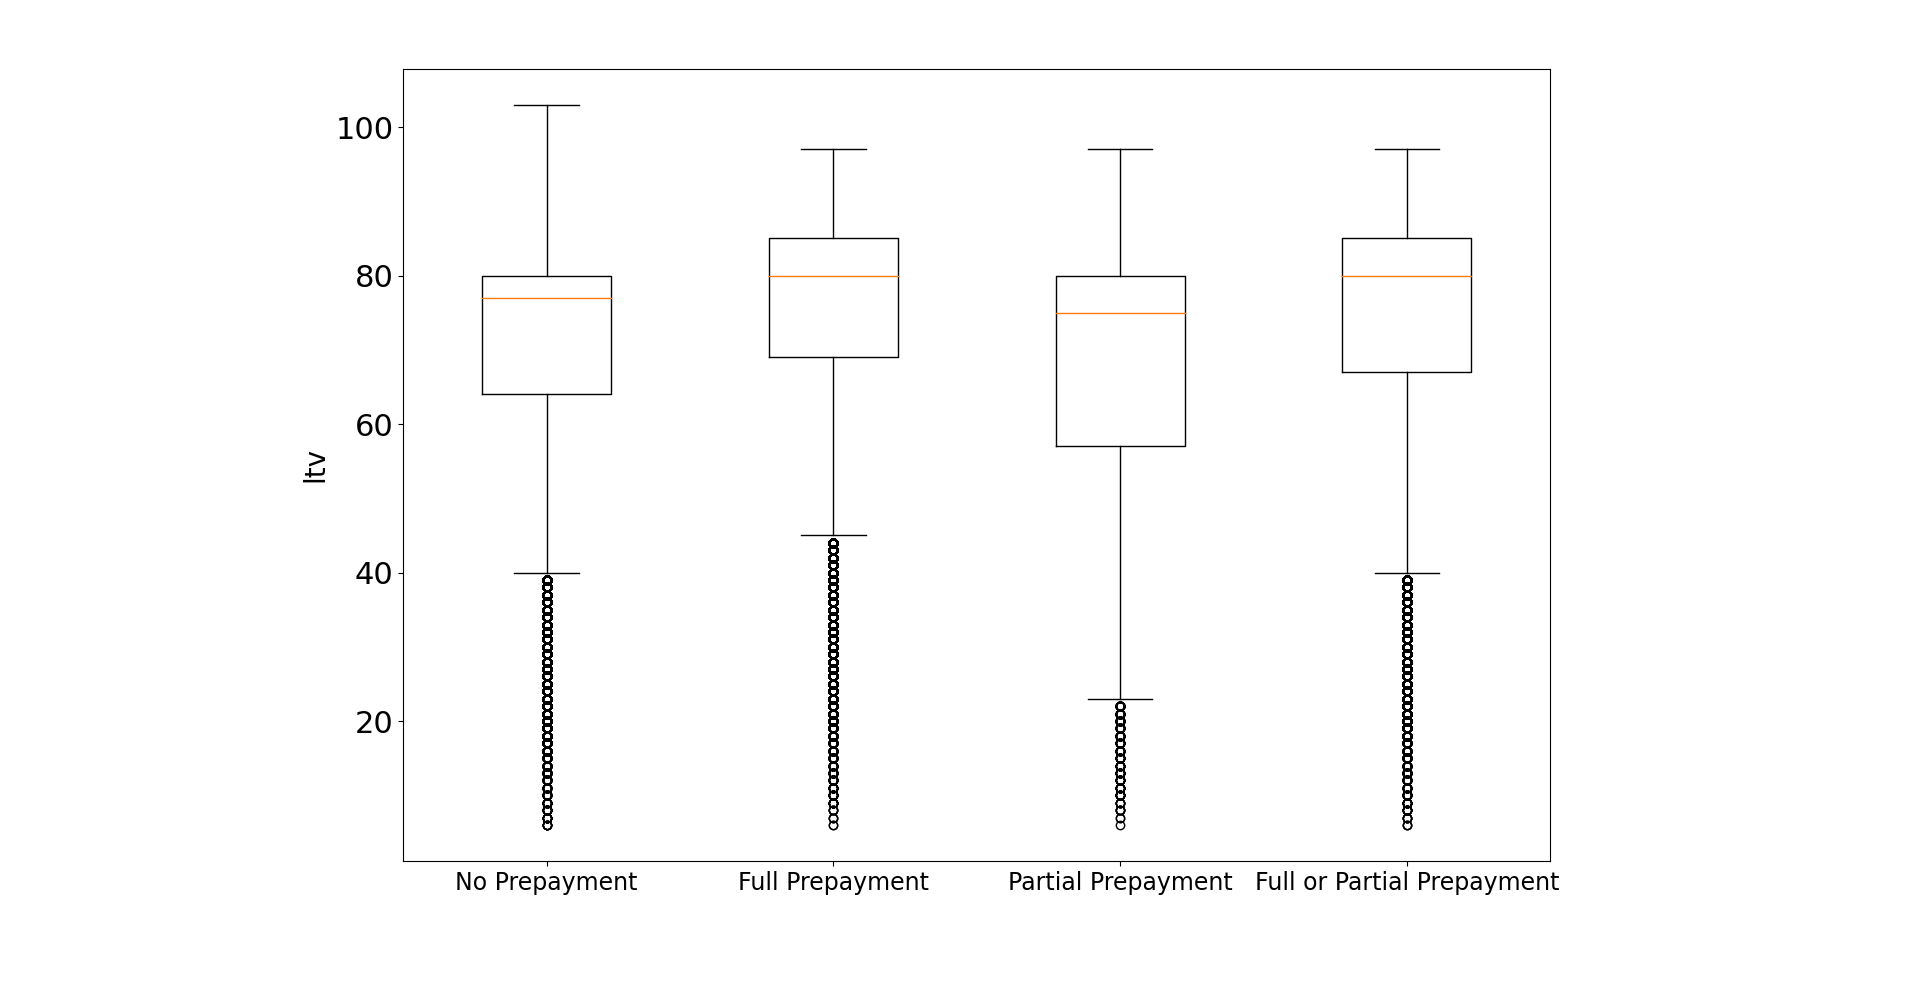
\includegraphics[width=\linewidth]{Figures/Boxplot_of_ltv_[2013, 2014, 2015, 2016, 2017, 2018, 2019, 2020]_.png}
            \caption{
                Boxplot of LTV for sample data.
                 From left to right: No prepayment, 
                 Full prepayment, Partial prepayment and Full or 
                 Partial prepayment.
                 }
            \label{model_boxplot_LTV}
        \end{figure}
        Combining Figure \ref{model_boxplot_LTV} and Table 
        \ref{model_Pvals_of_LTV}, LTV can be considered as a 
        potential risk driver and needs further investigation. One 
        observes similar behavior of the data through 
        the years. For further investigation, year 2013 is considered 
        as a separate year. This is possible as all years give similar 
        results.  
        \\\\
        In Figure \ref{model_LTV_against_prepayment} the loans in 
        which no prepayments are made are filtered out of the data. 
        From the figure, one can see that higher magnitudes of LTV  
        observed, values around 80, which is 
        in accordance with Figure \ref{model_boxplot_LTV}. This figures 
        implies again that LTV could be a risk driver. 
        \begin{figure}[H]
            \centering
            \begin{subfigure}{0.45\textwidth}
                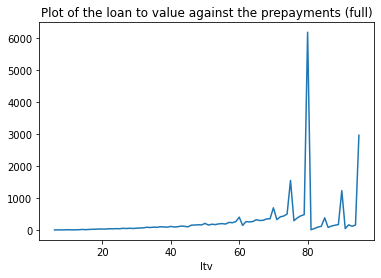
\includegraphics[width=\linewidth]{Figures/LTV againts Full prepayments.png}
                \caption{
                    LTV against Full prepayments.
                    }
                \label{model_LTV_against_full_prepayment}
            \end{subfigure}
            \begin{subfigure}{0.45\textwidth}
                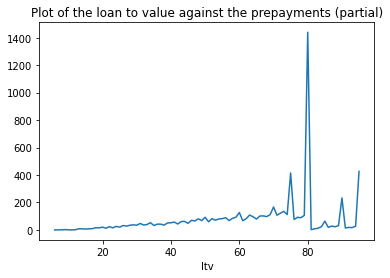
\includegraphics[width=\linewidth]{Figures/LTV againts Partial prepayments.png}
                \caption{
                    LTV against Partial prepayments.
                    }
                \label{model_LTV_against_partial_prepayment}
            \end{subfigure}
            \caption{LTV against magnitude of prepayments.}
            \label{model_LTV_against_prepayment}
        \end{figure}
    
    \subsubsection{Original combined loan-to-value}
        As stated, both CLTV and LTV are calculated in similar ways. 
        To study the behaviour of CLTV in case of partial and full 
        prepayments, a boxplot is made. In Figure \ref{model_boxplot_CLTV} 
        one obverses a difference in behaviour. This behaviour is tested 
        using Kolmogorov Smirnov test as well, the obtained $p$-values 
        can be found in Table \ref{model_Pvals_of_CLTV}. All $p$-values 
        are zero which suggest independent data. A zero $p$-value could 
        however, correspond to too much data, as well.
        \begin{table}[H]
        \centering
            \begin{tabular}{lcl|c|c}
                \multicolumn{3}{c|}{Prepayment type} 
                & P-values& KS-statistic \\\hline
                No Prepayment & \& & Full Prepayment & 0 & 0.070947\\
                No Prepayment & \& & Partial Prepayment & 0 & 0.090918\\
                No Prepayment & \& & Full or Partial Prepayment & 0 & 0.053969 \\
                Full Prepayment & \& & Partial Prepayment & 0 & 0.150986
		    \end{tabular}
            \caption{
                $p$-values of CLTV (in which if both partial and full 
                prepayments happen, it is denoted as full prepayment).
                }
	        \label{model_Pvals_of_CLTV}
        \end{table}
        Further investigating year 2013 one observes similar behaviour 
        for CLTV, see Figure \ref{model_CLTV_against_prepayment}. 
        This behavior is similar as with LTV.
        \begin{figure}[H]
            \centering
            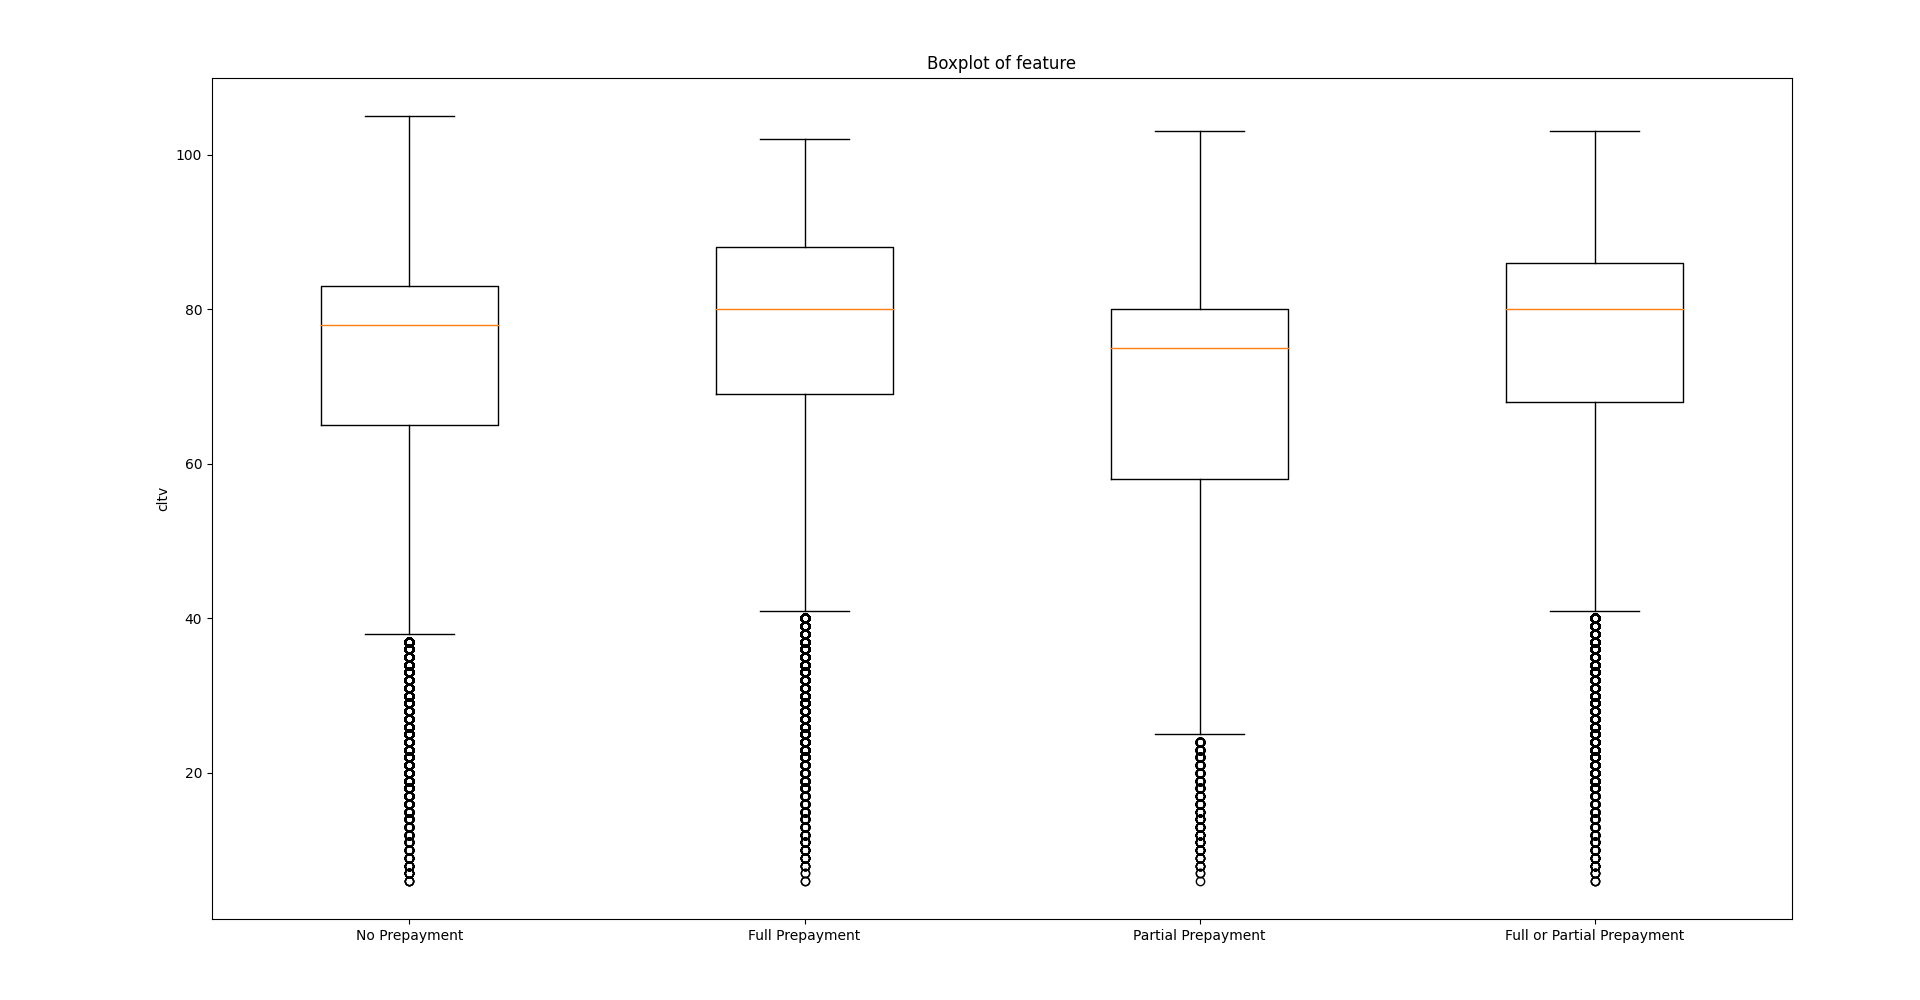
\includegraphics[width=\linewidth]{Figures/Boxplot_of_cltv_[2013, 2014, 2015, 2016, 2017, 2018, 2019, 2020]_.png}
            \caption{
                Boxplot of CLTV of sample data. From left to right: 
                No prepayment, Full prepayment, Partial prepayment 
                and Full or Partial prepayment.
                }
            \label{model_boxplot_CLTV}
        \end{figure}
        \begin{figure}[H]
            \centering
            \begin{subfigure}{0.45\textwidth}
                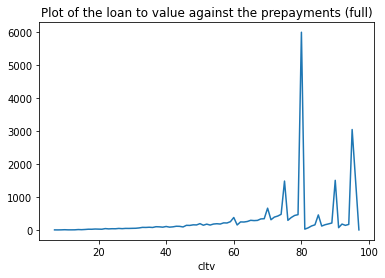
\includegraphics[width=\linewidth]{Figures/CLTV againts Full prepayments.png}
                \caption{
                    CLTV against Full prepayments.
                    }
                \label{model_CLTV_against_full_prepayment}
            \end{subfigure}
            \begin{subfigure}{0.45\textwidth}
                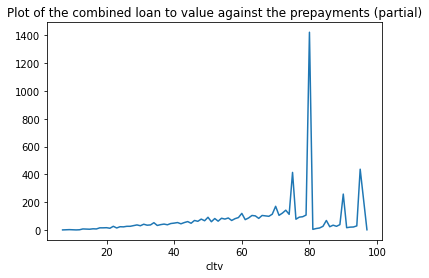
\includegraphics[width=\linewidth]{Figures/CLTV againts Partial prepayments.png}
                \caption{
                    CLTV against Partial prepayments.
                    }
                \label{model_CLTV_against_partial_prepayment}
            \end{subfigure}
            \caption{
                CLTV against magnitude of prepayments.
                }
            \label{model_CLTV_against_prepayment}
        \end{figure}

\subsubsection{Original interest rate}
    At last, the behaviour of characteristic original interest rate is 
    considered. It is expected that in loans with a higher interest 
    rate, more prepayments are made. This follows from getting a 
    loan somewhere else with lower interest rate and using this 
    money to prepay the original loan. The data is split based 
    on the kind of prepayment. This division is used to determine 
    possible dependence between this characteristic. The $p$-values 
    given in Table \ref{model_Pvals_of_int} suggest the data to 
    be independent. This test is performed on a large amount of 
    data and hence might be false. 
    \begin{table}[H]
        \centering
            \begin{tabular}{lcl|c|c}
                \multicolumn{3}{c|}{Prepayment type} & P-values& KS-statistic \\\hline
                No Prepayment & \& & Full Prepayment & 0 & 0.195919\\
                No Prepayment & \& & Partial Prepayment & 0 & 0.079967\\
                No Prepayment & \& & Full or Partial Prepayment & 0 & 0.165275 \\
                Full Prepayment & \& & Partial Prepayment & 0 & 0.263374
		    \end{tabular}
            \caption{
                $p$-values of interest rates (in which if both partial 
                and full prepayments happen, it is denoted as full 
                prepayment).
                }
	        \label{model_Pvals_of_int}
        \end{table}
    A boxplot comparing the prepayment might back up the $p$-values. 
    In Figure \ref{model_boxplot_int_rt}, a difference of behaviour 
    is seen based on the type of prepayment. A prepayment happens 
    more likely when the original interest rate is high. Which is 
    as expected. However, the partial prepayments turn out to be 
    made with smaller original interest rates. 
    \begin{figure}[H]
        \centering
        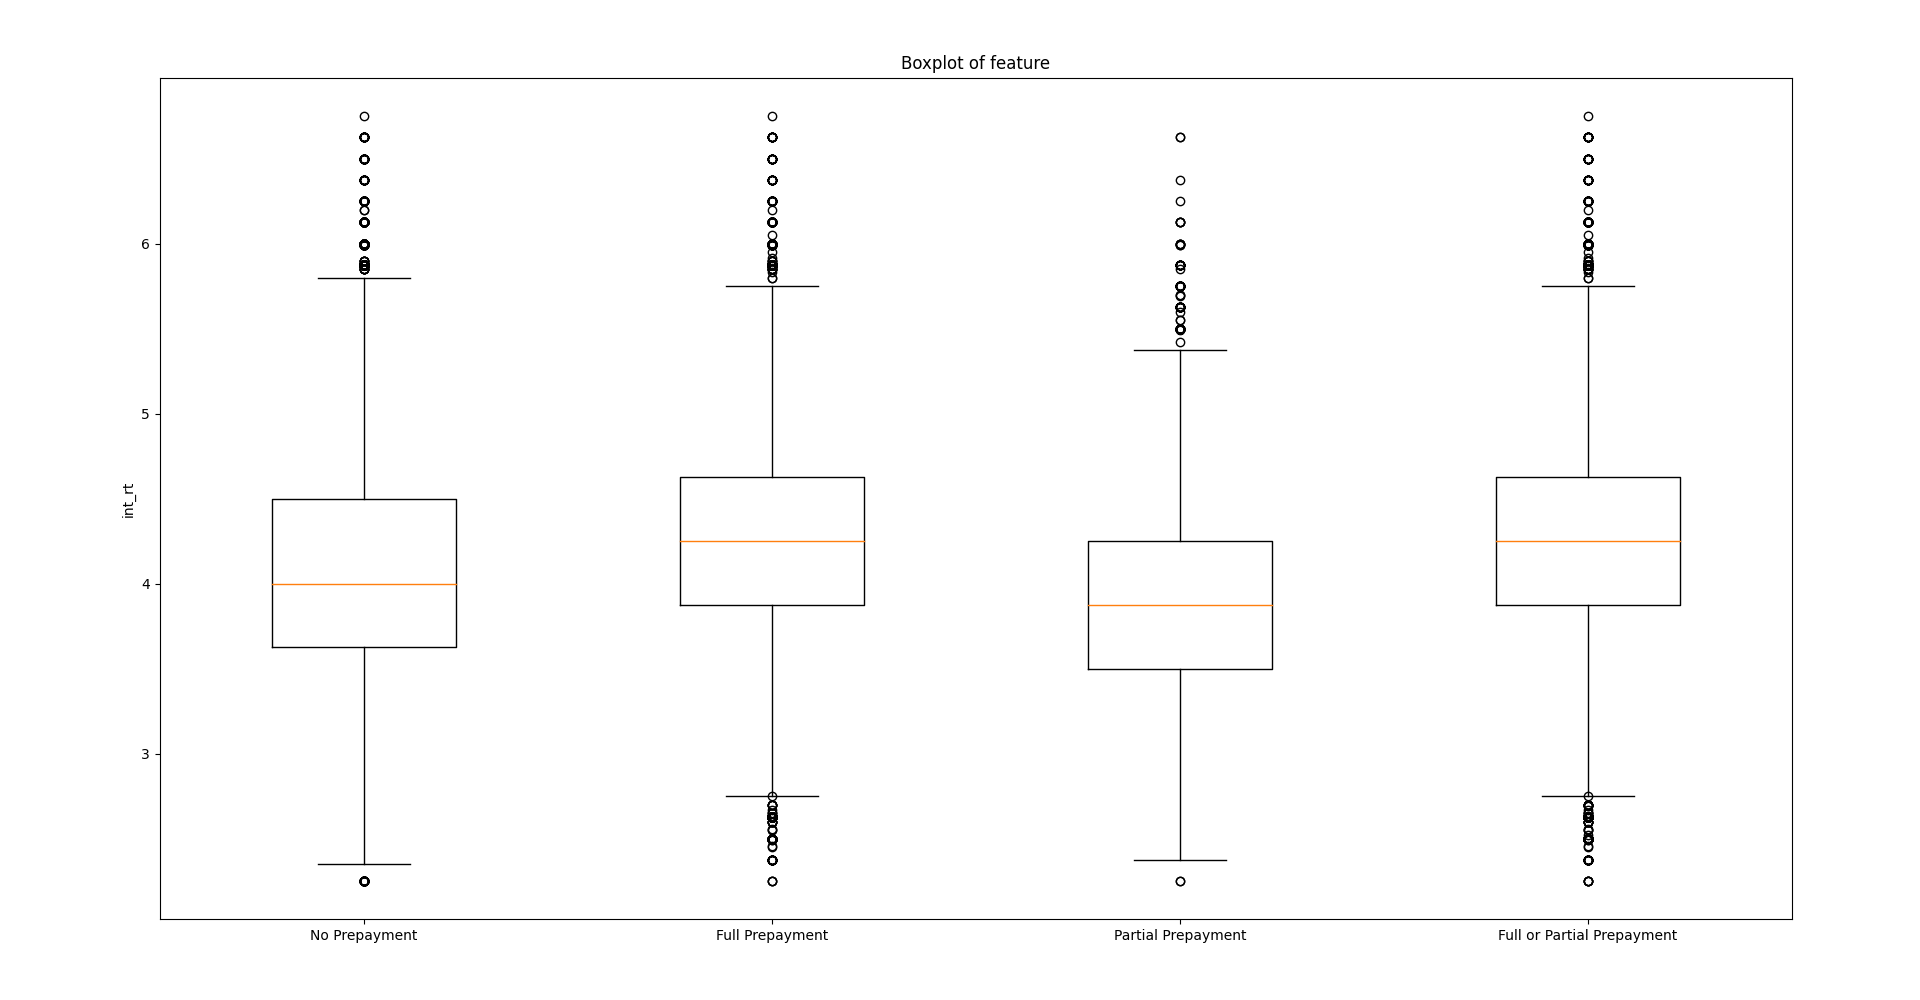
\includegraphics[width=\linewidth]{Figures/Boxplot_of_int_rt_[2013, 2014, 2015, 2016, 2017, 2018, 2019, 2020]_.png}
        \caption{
            Boxplot of original interest rate of sample data. 
            From left to right: No prepayment, Full prepayment, 
            Partial prepayment and Full or Partial prepayment.
            }
        \label{model_boxplot_int_rt}
    \end{figure}
    \noindent
    The influence of the original interest rate of year 2013 can be 
    seen in Figure \ref{model_int_rt_against_prepayment}. Here, 
    one observes again a higher interest rate implying more 
    prepayments. Note the interest rate for full prepayments to 
    be higher than the interest rate of partial prepayments. 
    \begin{figure}[H]
        \centering
        \begin{subfigure}{0.45\textwidth}
            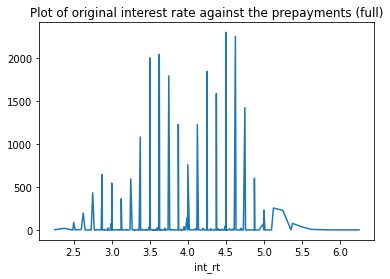
\includegraphics[width=\linewidth]{Figures/int_rt againts Full prepayments.png}
            \caption{
                Interest rate against Full prepayments.
                }
            \label{model_int_rt_against_full_prepayment}
        \end{subfigure}
        \begin{subfigure}{0.45\textwidth}
            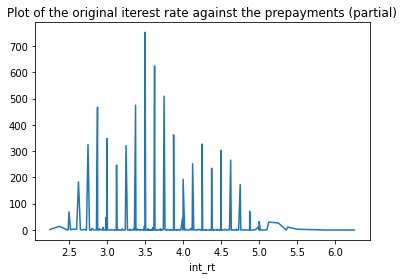
\includegraphics[width=\linewidth]{Figures/int_rt againts Partial prepayments.png}
            \caption{
                Interest rate against Partial prepayments.
                }
            \label{model_int_rt_against_partial_prepayment}
        \end{subfigure}
        \caption{
            Original interest rate against magnitude of prepayments.
            }
        \label{model_int_rt_against_prepayment}
    \end{figure}
        
\subsection{Interest incentive}
    We can further investigate the interest rate as a risk factor. 
    Together with the originating and monthly payments files we 
    also have access to the Mortgage US 15 over all the weeks 
    between 2013 an 2020. This gives us the fixed interest rate 
    that US home-buyers would pay if they take out a loan lasting 
    15 years at a certain time.
    \begin{figure}[H]
        \centering
        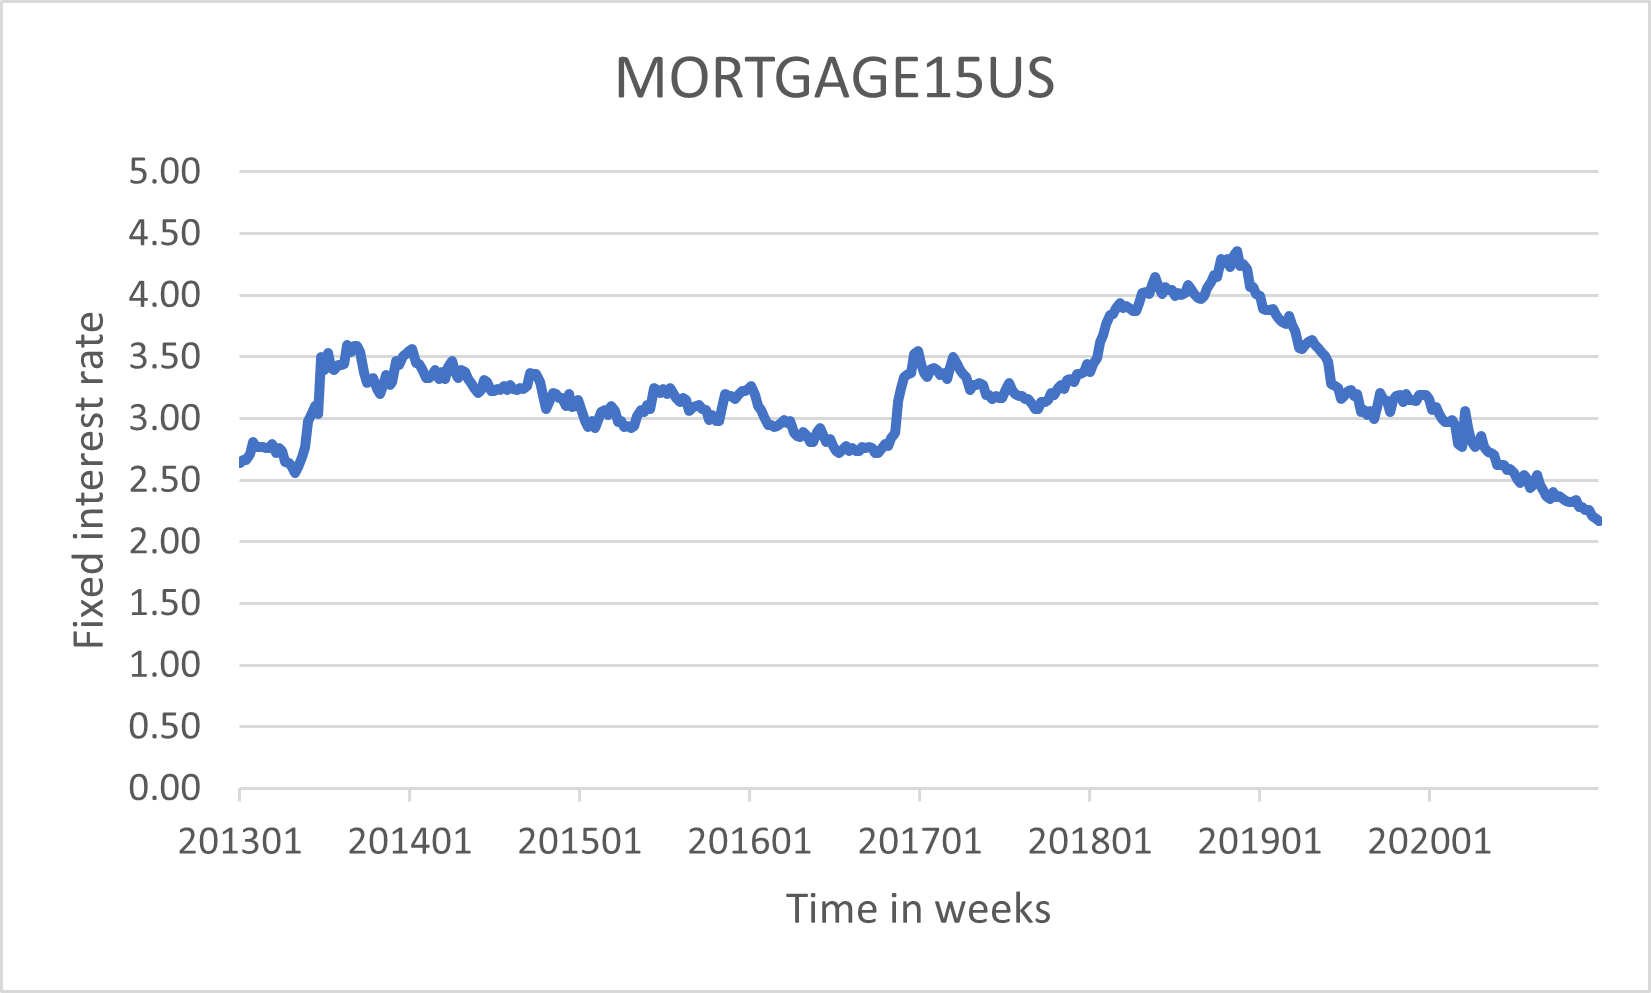
\includegraphics[scale=0.7]{Figures/mortgage15US.png}
        \caption{
            Graph of fixed interest rate in US
            }
        \label{mortgage15us}
    \end{figure}
    The fixed interest rates for the beginning of a mortgage is 
    given to us per week. To determine the fixed interest rate 
    per month we take the maximum of the interest rates per week. 
    This values are also close to the fixed interest rates for 
    mortgages over 30 and 40 years, we can use this data to compare 
    with the loans of 30 and 40 years in our data set.
    \\\\
    We would expect when the interest rate of a loan is higher then 
    the fixed interest rate corresponding to that time, a loanee wants 
    to fully prepay his mortgage and take a new one for the lower 
    fixed interest rate. Of course the loanee must have the resources 
    to fully pay-off his loan. When the loanee does not have the 
    resources to fully prepay his mortgage, the loanee could make 
    a partial prepayment. To see this incentive as a risk factor we 
    first make a new variable: \textit{the interest incentive}. 
    The interest incentive is defined as the current interest rate 
    of the loan minus the fixed interest for that given time. 
    When the interest incentive is positive we expect that the loanee 
    might make a prepayment. To see how the interest incentive 
    is related to the prepayments we look at figure 
    \ref{pvals_incentive}. 
    \\\\
    The box plots shows that there is significant difference in 
    the behaviour of the interest incentive in months with no 
    prepayment compared to full prepayments. Besides, performing 
    a Kolmogorov Smirnov test and obtain the p-values as given 
    in Table \ref{pvals_incentive}. All p-values are zero implying 
    independent data. A zero p-value could however, also correspond 
    to too much data. 
    However, we do not see a clear difference between no 
    prepayments en the partial prepayments. So we assume that 
    the interest incentive only has effect on full prepayment 
    which sounds logical. If a loanee does not have enough 
    resources to fully prepay the loan, apparently it is not 
    interesting for them to do a partial prepayment. We will 
    now further investigate the relationship between the 
    interest rate incentive and the full prepayments.

    \begin{table}[H]
    \centering
        \begin{tabular}{lcl|c|c}
            \multicolumn{3}{c}{Prepayment type} & $p$-values& KS-statistic \\\hline
            No Prepayment & \& & Full Prepayment & 0 & 0.208387\\
            No Prepayment & \& & Partial Prepayment & 0 & 0.083474\\
            No Prepayment & \& & Full or Partial Prepayment & 0 & 0.0567477 \\
            Full Prepayment & \& & Partial Prepayment & 0 & 0.275293
	    \end{tabular}
        \caption{
            $p$-values of interest incentive.
            }
	    \label{pvals_incentive}
    \end{table}

    \begin{figure}[H]
        \centering
        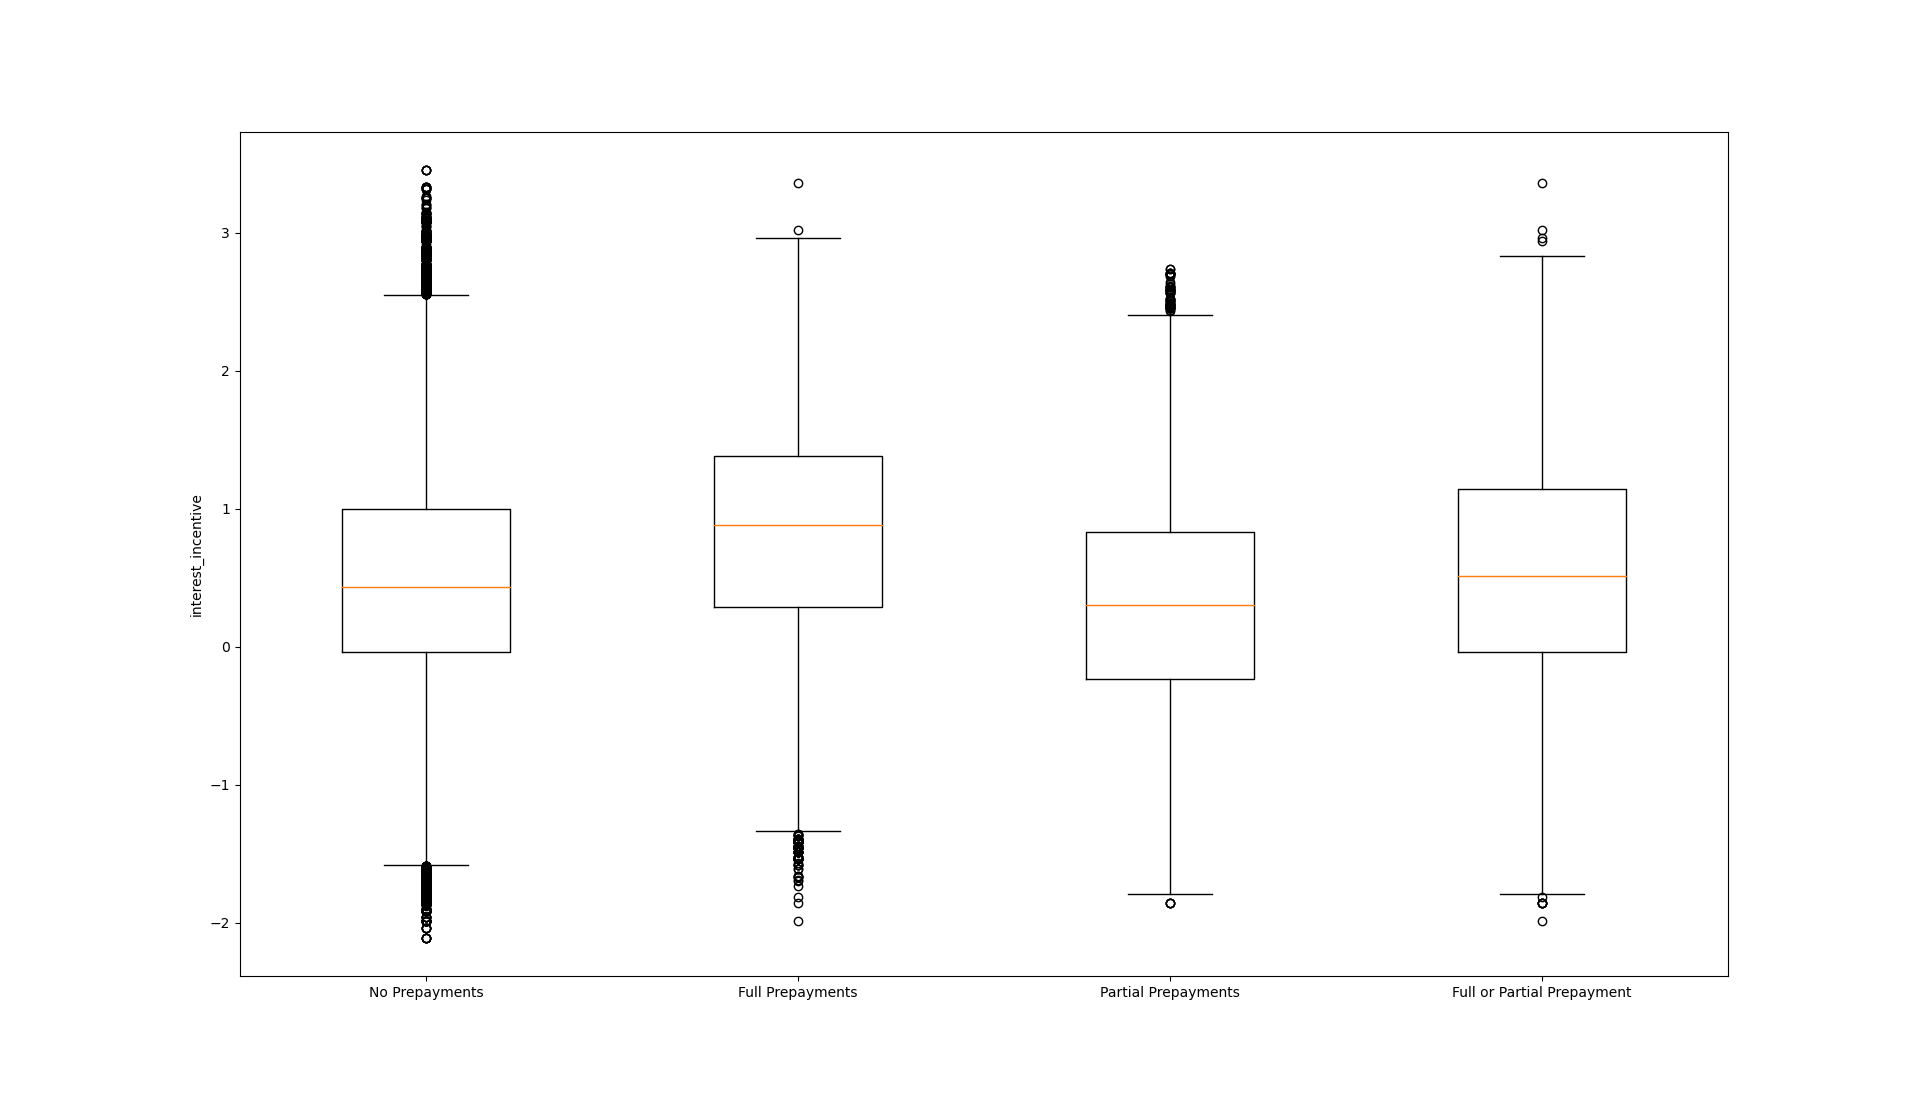
\includegraphics[width=\linewidth]{Figures/Boxplots_interest_incentive.png}
        \caption{
            Boxplot of interest incentive for sample data. From 
            left to right: No prepayment, Full prepayment, Partial 
            prepayment and Full or Partial prepayment.}
        \label{boxplots_incentive}
    \end{figure}
        
    To further investigate the relation between full prepayments and 
    the interest incentive we want to take a look at the observed 
    prepayment ratio. This is the ratio between the amount of debt 
    which is full prepaid over all the loans and the total outstanding 
    debt per month. This gives us a new variable which is unique per 
    month. We can now take a look at the relation between this ratio 
    and the interest incentive. We would expect that when the 
    interest incentive goes up, this ratio will to. 
    \\\\
    We will visualize this relation with a scatter plot, where each 
    dot will be bigger for the number of observations. Per different 
    values of the ratio we will look at the corresponding interest 
    rate incentives. The dot will then be placed on the mean of all 
    these incentives. The size of the dot will be determined by the 
    amount of interest incentive where this mean is based on. This 
    results in a clear plot as seen in Figure \ref{scatter_interest}.
    \begin{figure}[H]
        \centering
        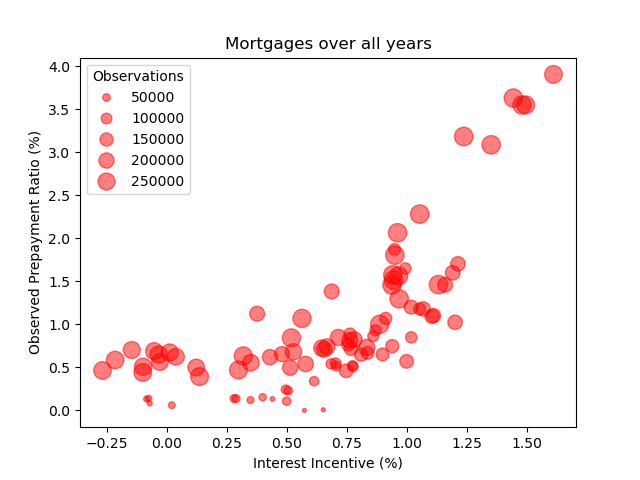
\includegraphics[scale=0.7]{Figures/Bubbles_all_years.png}
        \caption{Scatter plot of the observed prepayment ratio against the incentive interest.}
        \label{scatter_interest}
    \end{figure}
    From this we can conclude that the interest incentive does have 
    a clear effect on the observed prepayment ratio. We do still 
    see that with a negative interested incentive mortgage holders 
    do still prepay. This can be because of all different reasons. 
    The loanne could have had a equity injection or OTHER REASONS??!!